\documentclass{standalone}

% graphics
\usepackage{tikz}
\usepackage{pgfplots}
\usepackage{siunitx}

\begin{document}

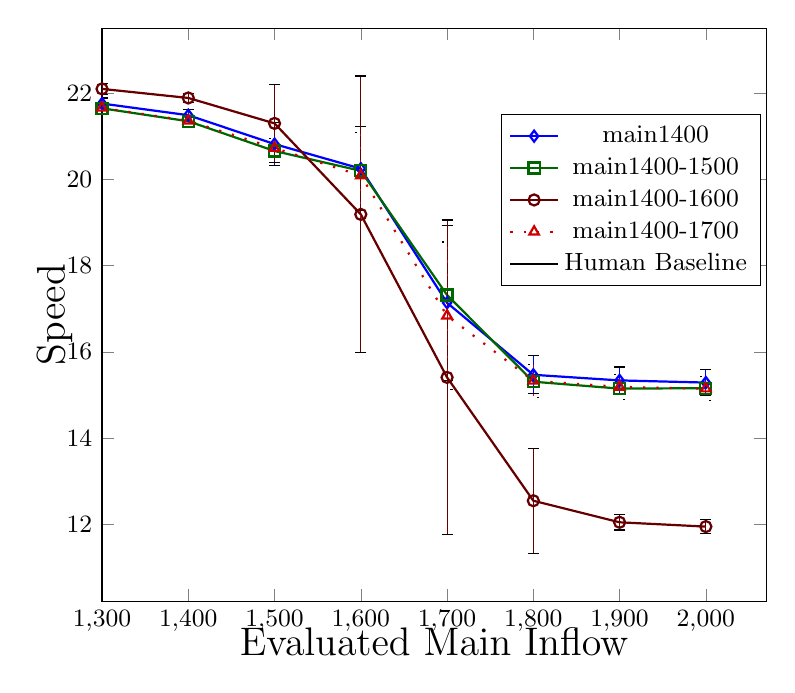
\begin{tikzpicture}[scale=1]
  \pgfplotsset{
      scale only axis,
      every x tick label/.append style={font=\small},
      every y tick label/.append style={font=\small},
	legend style={at={(0.6,0.85)},anchor=north west},
	xmin=1300
  }

\begin{axis}[
    legend style={font=\small},
	ylabel={\Large Speed},
	x label style={at={(axis description cs:0.5,-0.03)},anchor=north},
	y label style={at={(axis description cs:-0.030,0.5)}, anchor=south},
	xlabel={\Large Evaluated Main Inflow},
]




%main1400-1400_merge200
% dashdotdotted,
\addplot[mark=diamond, thick, mark options={solid, fill=blue!40, mark size=2 pt}, draw=blue, error bars/.cd, y dir=both, y explicit] table [x=a, y=b, y error=c] {
a	b   	c
1300 21.76 0.13
1400 21.49 0.14
1500 20.82 0.50
1600 20.25 0.97
1700 17.14 1.80
1800 15.47 0.44
1900 15.34 0.31
2000 15.29 0.31
};
\label{main1400}

%main1400-1500_merge200
% error bars/.cd, y dir=both, y explicit,
\addplot[mark=square, thick, mark options={solid, fill=green!60, mark size=2 pt}, draw=black!60!green] table [x=a, y=b] {
a	b   	c
1300 21.65 0.14
1400 21.35 0.14
1500 20.66 0.35
1600 20.20 0.53
1700 17.32 1.60
1800 15.31 0.36
1900 15.15 0.30
2000 15.16 0.30
};
\label{main1400-1500}  

%densely dashed, 
%main1400-1600_merge200
\addplot[mark=o, thick, mark options={solid, fill=black!60!red, mark size=2pt}, draw=black!60!red, error bars/.cd, y dir=both, y explicit] table [x=a, y=b, y error=c] {
a	b   	c
1300 22.10 0.12
1400 21.89 0.11
1500 21.30 0.90
1600 19.19 3.21
1700 15.41 3.65
1800 12.55 1.22
1900 12.05 0.18
2000 11.95 0.16
};
\label{main1400-1600}

%densely dashed, 
%main1400-1700_merge200
\addplot[mark=triangle, thick, loosely dotted, mark options={solid, fill=red!60, mark size=2pt}, draw=black!20!red, error bars/.cd, y dir=both, y explicit] table [x=a, y=b, y error=c] {
a	b   	c
1300 21.66 0.14
1400 21.36 0.14
1500 20.73 0.21
1600 20.09 1.00
1700 16.84 1.71
1800 15.33 0.38
1900 15.19 0.29
2000 15.15 0.28
};
\label{main1400-1700}

%%densely dashed, 
%\addplot[mark=otimes, thick, mark options={solid, fill=red!60, mark size=2pt},
%draw=blue!10!green, error bars/.cd, y dir=both, y explicit] table [x=a, y=b, y error=c] {
%a	b   	c
%2 9.26 0.25
%4 9.48 0.20
%6 9.95 0.27
%8 10.28 0.24
%10 10.80 0.18
%20 13.91 0.36
%30 15.48 0.22
%40 16.22 0.27
%50 16.99 0.36
%60 17.60 0.36
%70 17.93 0.29
%80 18.12 0.23
%90 18.20 0.18
%100 18.21 0.18
%};
%\label{AVP90}
%
%
%%densely dashed, 
%\addplot[mark=otimes, thick, mark options={solid, fill=blue!60, mark size=2pt},
%draw=blue!10!red, error bars/.cd, y dir=both, y explicit] table [x=a, y=b, y error=c] {
%a	b   	c
%2 7.26 0.15
%4 7.24 0.15
%6 7.27 0.15
%8 7.30 0.18
%10 7.34 0.18
%20 7.55 0.17
%30 7.91 0.29
%40 8.41 0.44
%50 9.19 0.69
%60 10.73 0.76
%70 11.74 0.68
%80 12.37 0.67
%100 13.57 0.64 
%};
%\label{linearPPO}


\addplot[mark=none, black, samples=200] coordinates {(0,16.27) (100,16.27)};{};\label{Baseline}

\addlegendimage{/pgfplots/refstyle=main1400}
\addlegendentry{main1400}

\addlegendimage{/pgfplots/refstyle=main1400-1500}
\addlegendentry{main1400-1500}

\addlegendimage{/pgfplots/refstyle=main1400-1600}
\addlegendentry{main1400-1600}

\addlegendimage{/pgfplots/refstyle=main1400-1700}
\addlegendentry{main1400-1700}

%\addlegendimage{/pgfplots/refstyle=AVP90}
%\addlegendentry{AVP90}

%\addlegendimage{/pgfplots/refstyle=linearPPO}
%\addlegendentry{linearPPOAVP10}

\addlegendimage{/pgfplots/refstyle=Baseline}
\addlegendentry{Human Baseline}




\end{axis}
\end{tikzpicture}

\end{document}

